\section{Monday}
\subsection{MSP --- Meridian Scanning Photometer}
\begin{enumerate}[\(\bullet \)]
    \item 30° off Meridional line since we want mag.\ mer.\ line.
    \item 4 photometers
    \item photon multiplier tube\begin{enumerate}[\(\triangleright \)]
        \item acc.\ electrons
        \item sees individual photons
        \item is cooled down to \SI{-20}{\celsius} to reduce thermal noise
    \end{enumerate}
\end{enumerate}

\subsection{Auroral forecast}
\begin{enumerate}[\(\bullet \)]
    \item Look at DSCOVR data
    \item \(B_z\) most influential
    \item \(B_y\) to affect polar cap convection pattern\begin{enumerate}[\(\triangleright \)]
        \item L1 at \(\num{1.5e9}\si{\metre}\). Solar wind: \SI{400}{\kilo\metre\second^{-1}}
        \item \(\rightarrow 1\) Hour
    \end{enumerate}
    \item Now look at SuperDARN to find convection time
    \item Typical convection speed: \(v_c\sim 300-\SI{500}{\metre\second^{-1}}\)
    \item Distance: (ionosphere height is trivial at \num{200000}~\si{\kilo\metre})\begin{equation*}
        30\degree \rightarrow\frac{\pi}{2}\frac{1}{3}\Rightarrow d=\frac{\pi}{6}R_E,\quad R_E=\SI{6600}{\kilo\metre}
    \end{equation*}
    \item Time:\begin{equation*}
        t=\frac{\pi}{6}\frac{R_E}{v_c}\approx \SI{8639}{\second}\approx 2.4\tn{ h},\quad v_c=\SI{400}{\metre\second^{-1}}
    \end{equation*}
\end{enumerate}
\begin{figure}[ht]
    \centering
    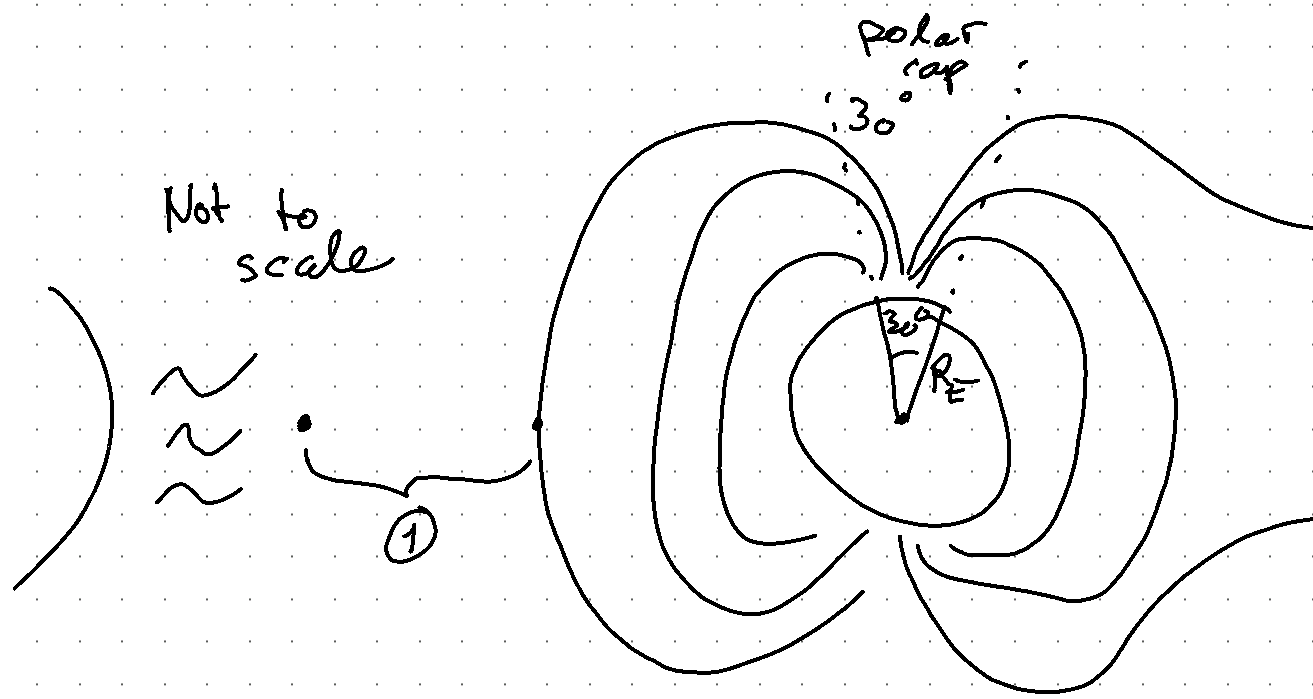
\includegraphics[width=.7\linewidth]{bilder/L5_field_work_monday.png}
    \caption{}\label{fig:L5_field_work_monday}
\end{figure}

\section{Tuesday}
Trigonometry the whole day more or less.

\section{Wednesday}
\subsection{The 1m GREEN}
\begin{enumerate}[\(\bullet \)]
    \item has a \SI{1}{\milli\metre} slit, and the narrower it is the higher the resolution, but you will also get less light in
    \item the angle the light enters the grating at is \SI{6.735}{\degree} from the normal
    \item blaze angle for the grating is \SI{30}{\degree}
    \item scans from \(420-\SI{430}{\nano\metre}\) which is where the Nitrogen line are located, and from \(480-\SI{490}{\nano\metre}\) where the Hydrogen \(H_\beta \) is part of the Balmer series
    \item for the most efficiency, we look for angles close to the blaze angle for how tilted he grating is\begin{enumerate}[\(\triangleright \)]
        \item 2.\ order for the \(H_\beta \) (\SI{36}{\degree}) where it has a \(\SI{3}{\angstrom/\milli\metre}\) resolution\begin{equation*}
            \fracd[x]{\lambda}=3.0\frac{\si{\angstrom}}{\si{\milli\metre}}
        \end{equation*}
    \end{enumerate}
\end{enumerate}

\section{Thursday}
\subsection{Absolute calibration}
\begin{enumerate}[\(\bullet \)]
    \item done once a year
    \item goal is to convert data into a usable unit
    \item set up shown in \cref{fig:L5_field_work_thursday}
\end{enumerate}
\begin{figure}[t]
    \centering
    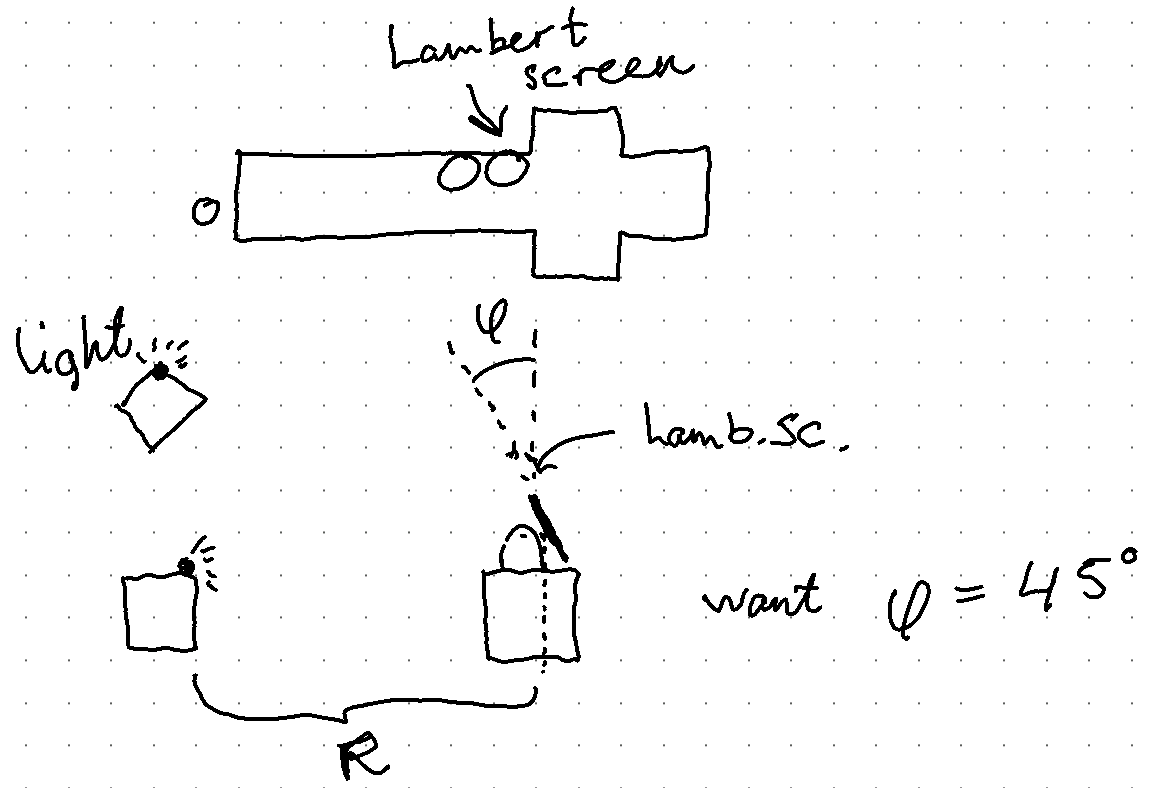
\includegraphics[width=.8\linewidth]{bilder/L5_field_work_thursday.png}
    \caption{Set up of the Tungsten lamp relative to the domes at KHO.}\label{fig:L5_field_work_thursday}
\end{figure}
So how do we do the conversion? If \(B_{ph}\) is the is the true luminance in SI units, then
\begin{equation*}
    B_{ph}=I_R\frac{1}{4\pi}10^4~\left[\frac{\tn{photon}}{\si{\metre^2\second}\ \tn{sr}}\right]
\end{equation*}
where ``sr'' stands for ``steradian'', a sort of 3D radian. The lamp that is used is a Tungsten lamp. The filament of the lamp will glow if you put a current through it and a voltage over it, and then for a given interval of wavelengths the intensity \(B_0(\lambda)\) will increase linearly with wavelength. A typical temperature in the filament is \(1000-\SI{2000}{\kelvin}\), with \SI{1000}{\kelvin} being associated with a red- yellow-ish color and \SI{2000}{\kelvin} being associated with more of a white color. We let \(B_0(\lambda)\) denote the known intensity, given in \si{\ray/\angstrom} at a known distance \(r\) (often \SI{1}{\metre}). Then the intensity \(B'(\lambda)\) at a distance \(R\) from the lamp is given by
\begin{equation*}
    B'(\lambda)=B_0(\lambda){\left(\frac{r}{R}\right)}^2
\end{equation*}
The Lambert's cosine law will finally give us the intensity that is remitted from the Lambert surface at an angle \(\varphi \)
\coloredeq{eq:abs_calibration}{B (\lambda)=B_0(\lambda)\left(\frac{r}{R}\right)^2\cos(\varphi)\rho}
where \(\rho \) is the diffuse reflectance factor, \(\rho=0.98\) in our case. If we now let \(C(\lambda)\) be the number of counts per second that is measured from the Tungsten lamp, and we have a measured auroral intensity \(I_A(\lambda)\) (both in unit \(\left[\tn{counts}/\tn{second}\right]\)), the intensity in absolute unit is given by
\begin{equation*}
    I(\lambda)=\frac{B(\lambda)}{C(\lambda)}I_A(\lambda)
\end{equation*}

\section{The aftermath}
\begin{enumerate}[\(\bullet \)]
    \item Looks like omega bands at 16:44:31 UT in the Sony a7s All Sky
    \item Two substorms in the evening, one starting at \(\sim \)18:00 UT and one from \(\sim \)21:40 UT
    \item Auroral arc reached as high in latitude as zenith for three substorms, as seen in sCMOS and also visible in Sony a7s All Sky
\end{enumerate}